



%%%%%%%%%%%%%%%%%%%%%%%%%%%%%%%%%%%%%%%%%
% Beamer Presentation
% LaTeX Template
% Version 1.0 (10/11/12)
%
% This template has been downloaded from:
% http://www.LaTeXTemplates.com
%
% License:
% CC BY-NC-SA 3.0 (http://creativecommons.org/licenses/by-nc-sa/3.0/)
%
%%%%%%%%%%%%%%%%%%%%%%%%%%%%%%%%%%%%%%%%%

%----------------------------------------------------------------------------------------
%	PACKAGES AND THEMES
%----------------------------------------------------------------------------------------

\documentclass[aspectratio=169]{beamer}

\mode<presentation> {


% The Beamer class comes with a number of default slide themes
% which change the colors and layouts of slides. Below this is a list
% of all the themes, uncomment each in turn to see what they look like.

%\usetheme{default}
%\usetheme{AnnArbor}
%\usetheme{Antibes}
%\usetheme{Bergen}
%\usetheme{Berkeley}
%\usetheme{Berlin}
%\usetheme{Boadilla}
%\usetheme{CambridgeUS}
%\usetheme{Copenhagen}
%\usetheme{Darmstadt}
%\usetheme{Dresden}
%\usetheme{Frankfurt}
%\usetheme{Goettingen}
%\usetheme{Hannover}
%\usetheme{Ilmenau}
%\usetheme{JuanLesPins}
%\usetheme{Luebeck}
\usetheme{Madrid}
%\usetheme{Malmoe}
%\usetheme{Marburg}
%\usetheme{Montpellier}
%\usetheme{PaloAlto}
%\usetheme{Pittsburgh}
%\usetheme{Rochester}
%\usetheme{Singapore}
%\usetheme{Szeged}
%\usetheme{Warsaw}

% As well as themes, the Beamer class has a number of color themes
% for any slide theme. Uncomment each of these in turn to see how it
% changes the colors of your current slide theme.

%\usecolortheme{albatross}
%\usecolortheme{beaver}
%\usecolortheme{beetle}
%\usecolortheme{crane}
%\usecolortheme{dolphin}
%\usecolortheme{dove}
%\usecolortheme{fly}
%\usecolortheme{lily}
%\usecolortheme{orchid}
%\usecolortheme{rose}
%\usecolortheme{seagull}
%\usecolortheme{seahorse}
%\usecolortheme{whale}
%\usecolortheme{wolverine}

%\setbeamertemplate{footline} % To remove the footer line in all slides uncomment this line
%\setbeamertemplate{footline}[page number] % To replace the footer line in all slides with a simple slide count uncomment this line
\usepackage{amsmath}
\usepackage{selinput}      % Halbautomatische Auswahl der Eingabecodierung
\SelectInputMappings{      % mit Hilfe ausgewählter Glyphen
  adieresis={ä},	   % siehe: http://partners.adobe.com/public/developer/en/opentype/glyphlist.txt
  germandbls={ß},
  Euro={€}
}

\definecolor{UOSred}{rgb}{0.6745098039215686, 0.02352241176470588, 0.2039215686274510} % UBC Blue (primary)
\definecolor{UOSgrey}{rgb}{0.8117647058823522, 0.8117647058823522, 0.8117647058823522} % UBC Grey (secondary)

\setbeamercolor{palette primary}{bg=UOSred,fg=white}
\setbeamercolor{palette secondary}{bg=UOSred,fg=white}
\setbeamercolor{palette tertiary}{bg=UOSred,fg=white}
\setbeamercolor{palette quaternary}{bg=UOSred,fg=white}
\setbeamercolor{structure}{fg=UOSred} % itemize, enumerate, etc
\setbeamercolor{section in toc}{fg=UOSred} % TOC sections

%gets rid of bottom navigation bars
\setbeamertemplate{footline}[frame number]{}

%gets rid of bottom navigation symbols
\setbeamertemplate{navigation symbols}{}

\addtobeamertemplate{footline}{%
  \leavevmode%
  \hbox{%
  \begin{beamercolorbox}[wd=\paperwidth,ht=2.25ex,dp=1ex,center]{author in head/foot}%
     \insertsectionnavigationhorizontal{\paperwidth}{}{}
  \end{beamercolorbox}}%

}

% Override palette coloring with secondary
\setbeamercolor{subsection in head/foot}{bg=UOSgrey,fg=white}

%\setbeamertemplate{navigation symbols}{} % To remove the navigation symbols from the bottom of all slides uncomment this line
}
\usepackage{hyperref}
\usepackage{graphicx} % Allows including images
\usepackage{grffile}
\usepackage{booktabs} % Allows the use of \toprule, \midrule and \bottomrule in tables
\graphicspath{{images/}}
%----------------------------------------------------------------------------------------
%	TITLE PAGE
%----------------------------------------------------------------------------------------

\title[Aufgabe 4.3]{Aufgabe 5.3} % The short title appears at the bottom of every slide, the full title is only on the title page

\author{T. Adam, M. ben Ahmed} % Your name
\institute[UOS] % Your institution as it will appear on the bottom of every slide, may be shorthand to save space
{

Universität Osnabrück \\ % Your institution for the title page

\medskip
\textit{Æ} % Your email address


}
\date{\today} % Date, can be changed to a custom date

\begin{document}

\begin{frame}
\titlepage % Print the title page as the first slide
\end{frame}


%----------------------------------------------------------------------------------------
%	PRESENTATION SLIDES
%----------------------------------------------------------------------------------------


%------------------------------------------------

\begin{frame}
	\frametitle{Aufgabe 5.3 - Public Transport}
	\begin{columns}[c] % The "c" option specifies centered vertical alignment while the "t" option is used for top vertical alignment
		
		\column{.8\textwidth} % Left column and width
		\textbf{Intriguingly Simple and Fast Transit Routing (2013)}
		\begin{itemize}
			\item[]
			\item J. Dibbelt, T. Pajor, B. Strasser, D. Wagner
			\item Berechnen von optimalen Routen in öffentlichen Verkehrsnetzen
			\item[]
			\item Connection Scan Algorithmus (CSA)
			\begin{itemize}
				\item earliest arrival
				\item multi-criteria optimization
				\item minimum expected arrival time problem (MEAT)
			\end{itemize}

		\end{itemize}	
	\end{columns}
	\end{frame}
	
%------------------------------------------------

\begin{frame}
\frametitle{Grundbegriffe}
\begin{columns}[c] % The "c" option specifies centered vertical alignment while the "t" option is used for top vertical alignment
	
	\column{.5\textwidth} % Left column and width
	\textbf{Stops und Connections}
	\begin{itemize}
		\item Stops $p$
		\item Connections $c$
		\item $p_{dep}(c)$ Abfahrt-Stop
		\item $p_{arr}(c)$ Ankunft-Stop
		\item $\tau_{dep}(c)$ Abfahrtszeit von $c$
		\item $\tau_{arr}(c)$ Ankunftszeit von $c$
		\item $\tau_{ch}(p)$ Umstiegszeit an Stop $p$
	\end{itemize}
	\column{.3\textwidth} % Right column and width
	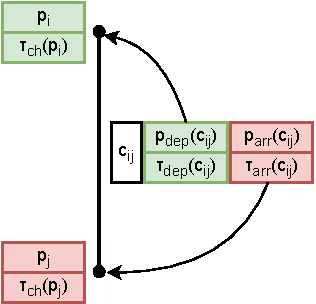
\includegraphics[scale=0.9]{connection.pdf}	
\end{columns}
\end{frame}

%------------------------------------------------


\begin{frame}
\frametitle{Grundbegriffe}
\begin{columns}[c] % The "c" option specifies centered vertical alignment while the "t" option is used for top vertical alignment
	
	\column{.6\textwidth} % Left column and width
	\textbf{Trips und Footpaths}
	\begin{itemize}
		\item Trip als Reihenfolge von Connections des selben Fahrzeugs
		\item $t(c)$ Trip von Connection $c$
		\item Footpath zwischen zwei nahegelegenen Stops
		\item Footpaths dürfen nicht auf einander folgen
		\item Routen als Mengen von Trips mit der selben Stop-Sequenz
	\end{itemize}
	\column{.3\textwidth} % Right column and width
	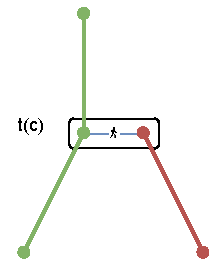
\includegraphics[scale=1.2]{trips_footpaths.pdf}	
\end{columns}
\end{frame}

%------------------------------------------------

\begin{frame}
\frametitle{Probleme}
\begin{columns}[c] % The "c" option specifies centered vertical alignment while the "t" option is used for top vertical alignment
	
	\column{.5\textwidth} % Left column and width
	\textbf{Earliest Arrival Problem}
	\begin{itemize}
		\item Gegeben:
		\begin{itemize}
			\item Startort und Startzeit
			\item Zielort
			\item Fahrplan mit Abfahrts- und Ankunftszeiten
		\end{itemize}
		\item Gesucht: Menge an Verbindungen (Route) \\ mit frühster Ankunftszeit
	\end{itemize}
	\column{.4\textwidth} % Right column and width
	
\includegraphics[scale=0.2]{bus.png}	
\end{columns}
\end{frame}

%------------------------------------------------


\begin{frame}
\frametitle{Connection Scan Algorithmus}
\begin{columns}[c] % The "c" option specifies centered vertical alignment while the "t" option is used for top vertical alignment
	
	\column{.6\textwidth} % Left column and width
	\textbf{Connection Scan Algorithmus}
	\begin{itemize}
		\item Array aller Connections nach Abfahrtszeit sortieren
		\item Für jeden Stop ein Label speichern (intial $\infty$)
		\item Über Connection Array iterieren und entsprechende Labels aktualisieren
		\item Beispiel mit 5 Stops und 4 Connections
	\end{itemize}
	\column{.3\textwidth} % Right column and width
	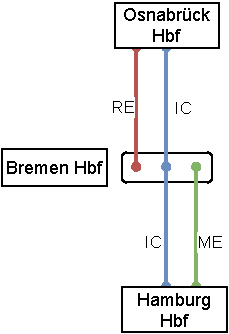
\includegraphics[scale=1]{csa_instance.pdf}
	
\end{columns}
\end{frame}

%------------------------------------------------

\begin{frame}
\frametitle{Connection Scan Algorithmus - Beispiel}
\centering
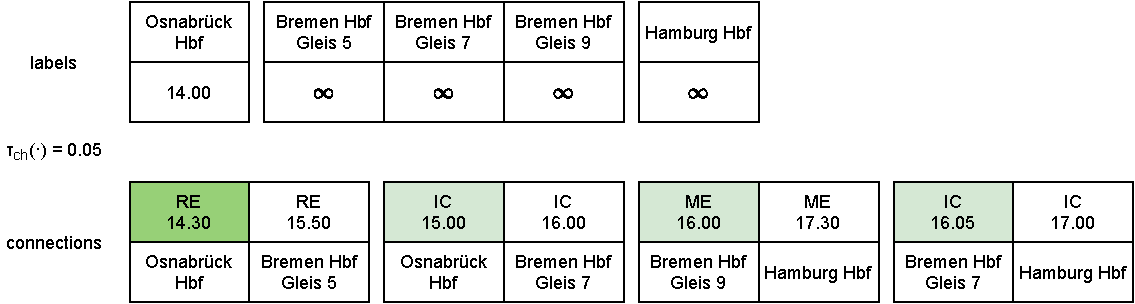
\includegraphics[scale=.7]{csa0.pdf}
\end{frame}

%------------------------------------------------

\begin{frame}
\frametitle{Connection Scan Algorithmus - Beispiel}
\centering
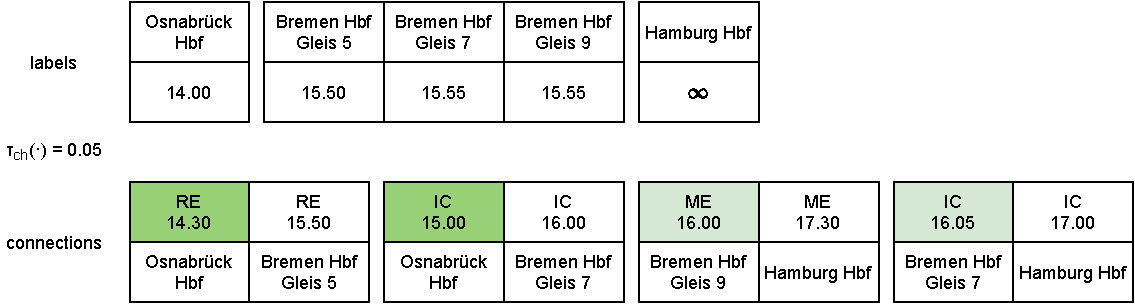
\includegraphics[scale=.7]{csa1.pdf}
\end{frame}

%------------------------------------------------

\begin{frame}
\frametitle{Connection Scan Algorithmus - Beispiel}
\centering
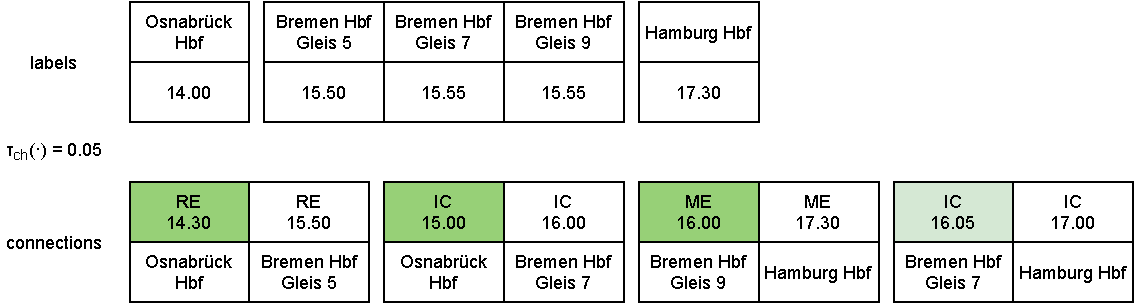
\includegraphics[scale=.7]{csa2.pdf}
\end{frame}

%------------------------------------------------

\begin{frame}
\frametitle{Connection Scan Algorithmus - Beispiel}
\centering
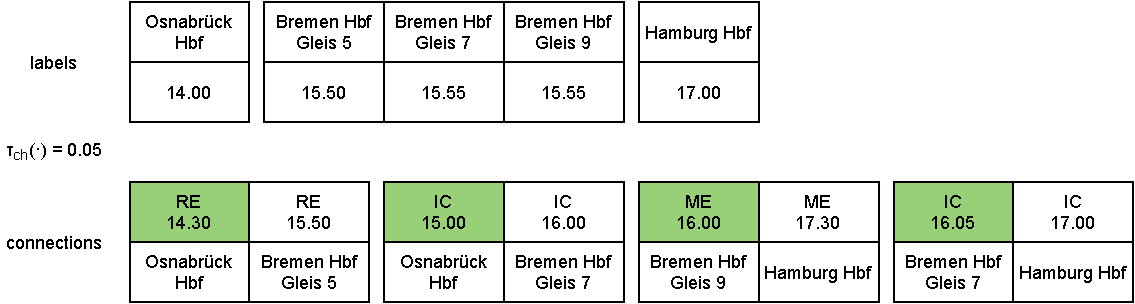
\includegraphics[scale=.7]{csa3.pdf}
\end{frame}

%------------------------------------------------
\begin{frame}
\frametitle{Erweiterungen}
\begin{columns}[c] % The "c" option specifies centered vertical alignment while the "t" option is used for top vertical alignment
	
	\column{.5\textwidth} % Left column and width
	\textbf{Profile Queries}
	\begin{itemize}
		\item Pareto Set
		\item Lösbar durch erweiterung von CSA durch dynamische Programmierung
	\end{itemize}
	\column{.4\textwidth} % Right column and width
	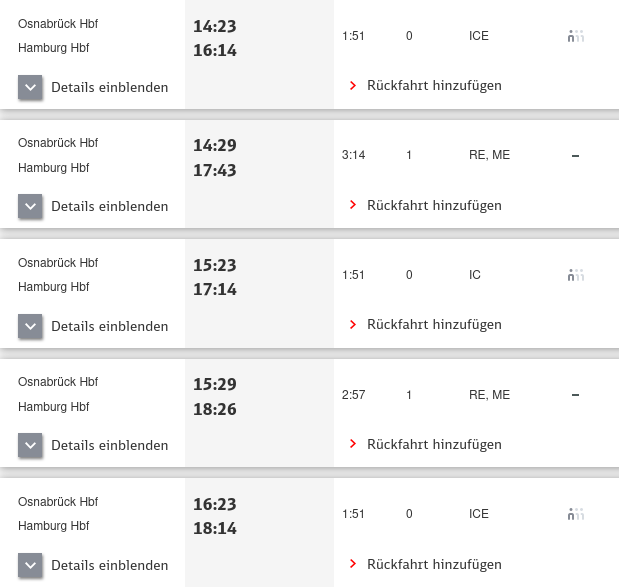
\includegraphics[scale=0.3]{profiles.png}
	
\end{columns}
\end{frame}

%------------------------------------------------


\end{document} 